\documentclass[sigconf,nonacm,prologue,table]{acmart}
\usepackage{listings}

%% labels
%% sections:    "sec"
%% definitions: "def"
%% equations:   "eq"
%% figures:     "fig"
%% tables:      "tab"

%% packages
\usepackage{amsmath}
\usepackage{pgfplots}
\usepackage{subcaption}
\usepackage{commath}
\usepackage[utf8]{inputenc}
\usetikzlibrary{positioning, arrows.meta, shapes, calc}
%% \usepackage{tikz}
\usepackage{graphicx}
\graphicspath{ {../docs/} }
\usepackage{afterpage}

\pagenumbering{arabic}

%% hide ACM reference
\settopmatter{printacmref=false}

%% hide copyright
\renewcommand\footnotetextcopyrightpermission[1]{}

%% \pagestyle{plain}
\settopmatter{printfolios=true}

\numberwithin{equation}{section}

\theoremstyle{definition}
\newtheorem{definition}{Definition}

\theoremstyle{remark}
\newtheorem*{remark}{Remark}

\captionsetup[subfigure]{
    labelfont=bf,
    textfont=normalfont,
}
\renewcommand{\thesubfigure}{\Roman{subfigure}}

\newcommand{\dshares}{\textsc{Dinari} d\textsc{Shares} }

\definecolor{rowA}{gray}{0.9}
\definecolor{rowB}{gray}{0.8}

\newcommand{\rplus}{\mathbb{R}_{\geq 0}}
\newcommand{\rpos}{\mathbb{R}_{>0}}

\begin{document}
\title{Dinari Securities Backed Tokens (dShares) v1 [Draft]}
\subtitle{June 2023}
\date{June 2023}

\author{Jake Timothy}
\affiliation{}
\email{jake@dinari.com}

\begin{teaserfigure}
\caption*{
    \hspace{\textwidth}
    }
\end{teaserfigure}

\renewcommand{\shortauthors}{Timothy}

\begin{abstract}

In order to realize the vision of blockchain technology enabling a more accessible, transparent, and secure system for the world’s quadrillions of dollars in derivatives and spot trading, a trusted bridge from the existing to the new platforms is required. We at Dinari built the Securities Backed Token (dShares) platform to be that trusted bridge. The dShares platform is a set of tokens backed 1-to-1 by existing publicly traded equities and a set of issuer smart contracts that process primary purchases and sales of those tokens. As orders are submitted, Dinari automatically rebalances it’s equities vaults, working with multiple clearing services, to maintain at least 100\% backing of the outstanding tokens.

\end{abstract}

\maketitle

\section{Introduction} \label{sec:introduction}

The Securities Backed Tokens are ERC-20 compliant and compatible with the full range of decentralized financial applications. The dShares platform is the first building block that we are releasing, with more on the way.

\section{The Tokens} 
\label{sec:Tokens}

We at Dinari have designed the Securities Backed Tokens to maximize interoperability with decentralized finance while maintaining security.

\subsection{Transfer Restrictions}

Dinari deploys one TransferRestrictor contract per issuing jurisdiction. All tokens backed by assets issued in one jurisdiction share a transfer restrictor. Tokens backed by assets issued in another jurisdiction may have different security requirements.

\subsection{Voting}

In order for the Security Backed Tokens to trade freely without onerous transfer restrictions, Dinari holds back shareholder voting rights from tokenholders.

Since the underlying securities are held by the Dinari Vault, the entire block of shares would need to vote together. In order to prevent unknown actors from accumulating voting power, tokenholders would register in order to cast their vote. We expect that for any shareholder vote, a small percentage of the overall token supply would register, complete a KYC process, and participate in voting. This would result in a small amount of tokens directing a potentially large block of voting power. For the time being, we have decided not to have token holders direct the Vault’s shareholder voting decisions.

\subsection{Dividends and Distributions}

SBT holders can earn dividends by registering. When dividends are announced for the underlying equity, token holdings are snapshot at the block corresponding to the designated distribution time. Distributions are deposited into a claim contract in USDC where accounts can withdraw up to their distribution amount.

\subsection{Proof of Reserves}

\section{Order Processors}
\label{sec:Processors}

The \dshares protocol operates like a bridge. Calls to official contracts inheriting from OrderProcessor emit orders. These orders are picked up by Dinari's fulfillment service, which executes an order through a clearing service. The clearing service then settles the order and notifies the fulfillment service. The fulfillment service then notifies the OrderProcessor contract that the order has been filled and dShares are minted or burned to the order recipient. Different order processing logic can be implemented. The IOrderBridge interface Order specification supports market and liimit orders.

\dshares v1 has implemented
\begin{itemize}
    \item An escrow locked market buy processor
    \item An escrow locked market sell processor
    \item An escrow unlocked market buy processor
\end{itemize}

% TODO: simplify sequence diagram
\afterpage{%
\begin{figure}
    \label{fig:order-processing}
    \centering
    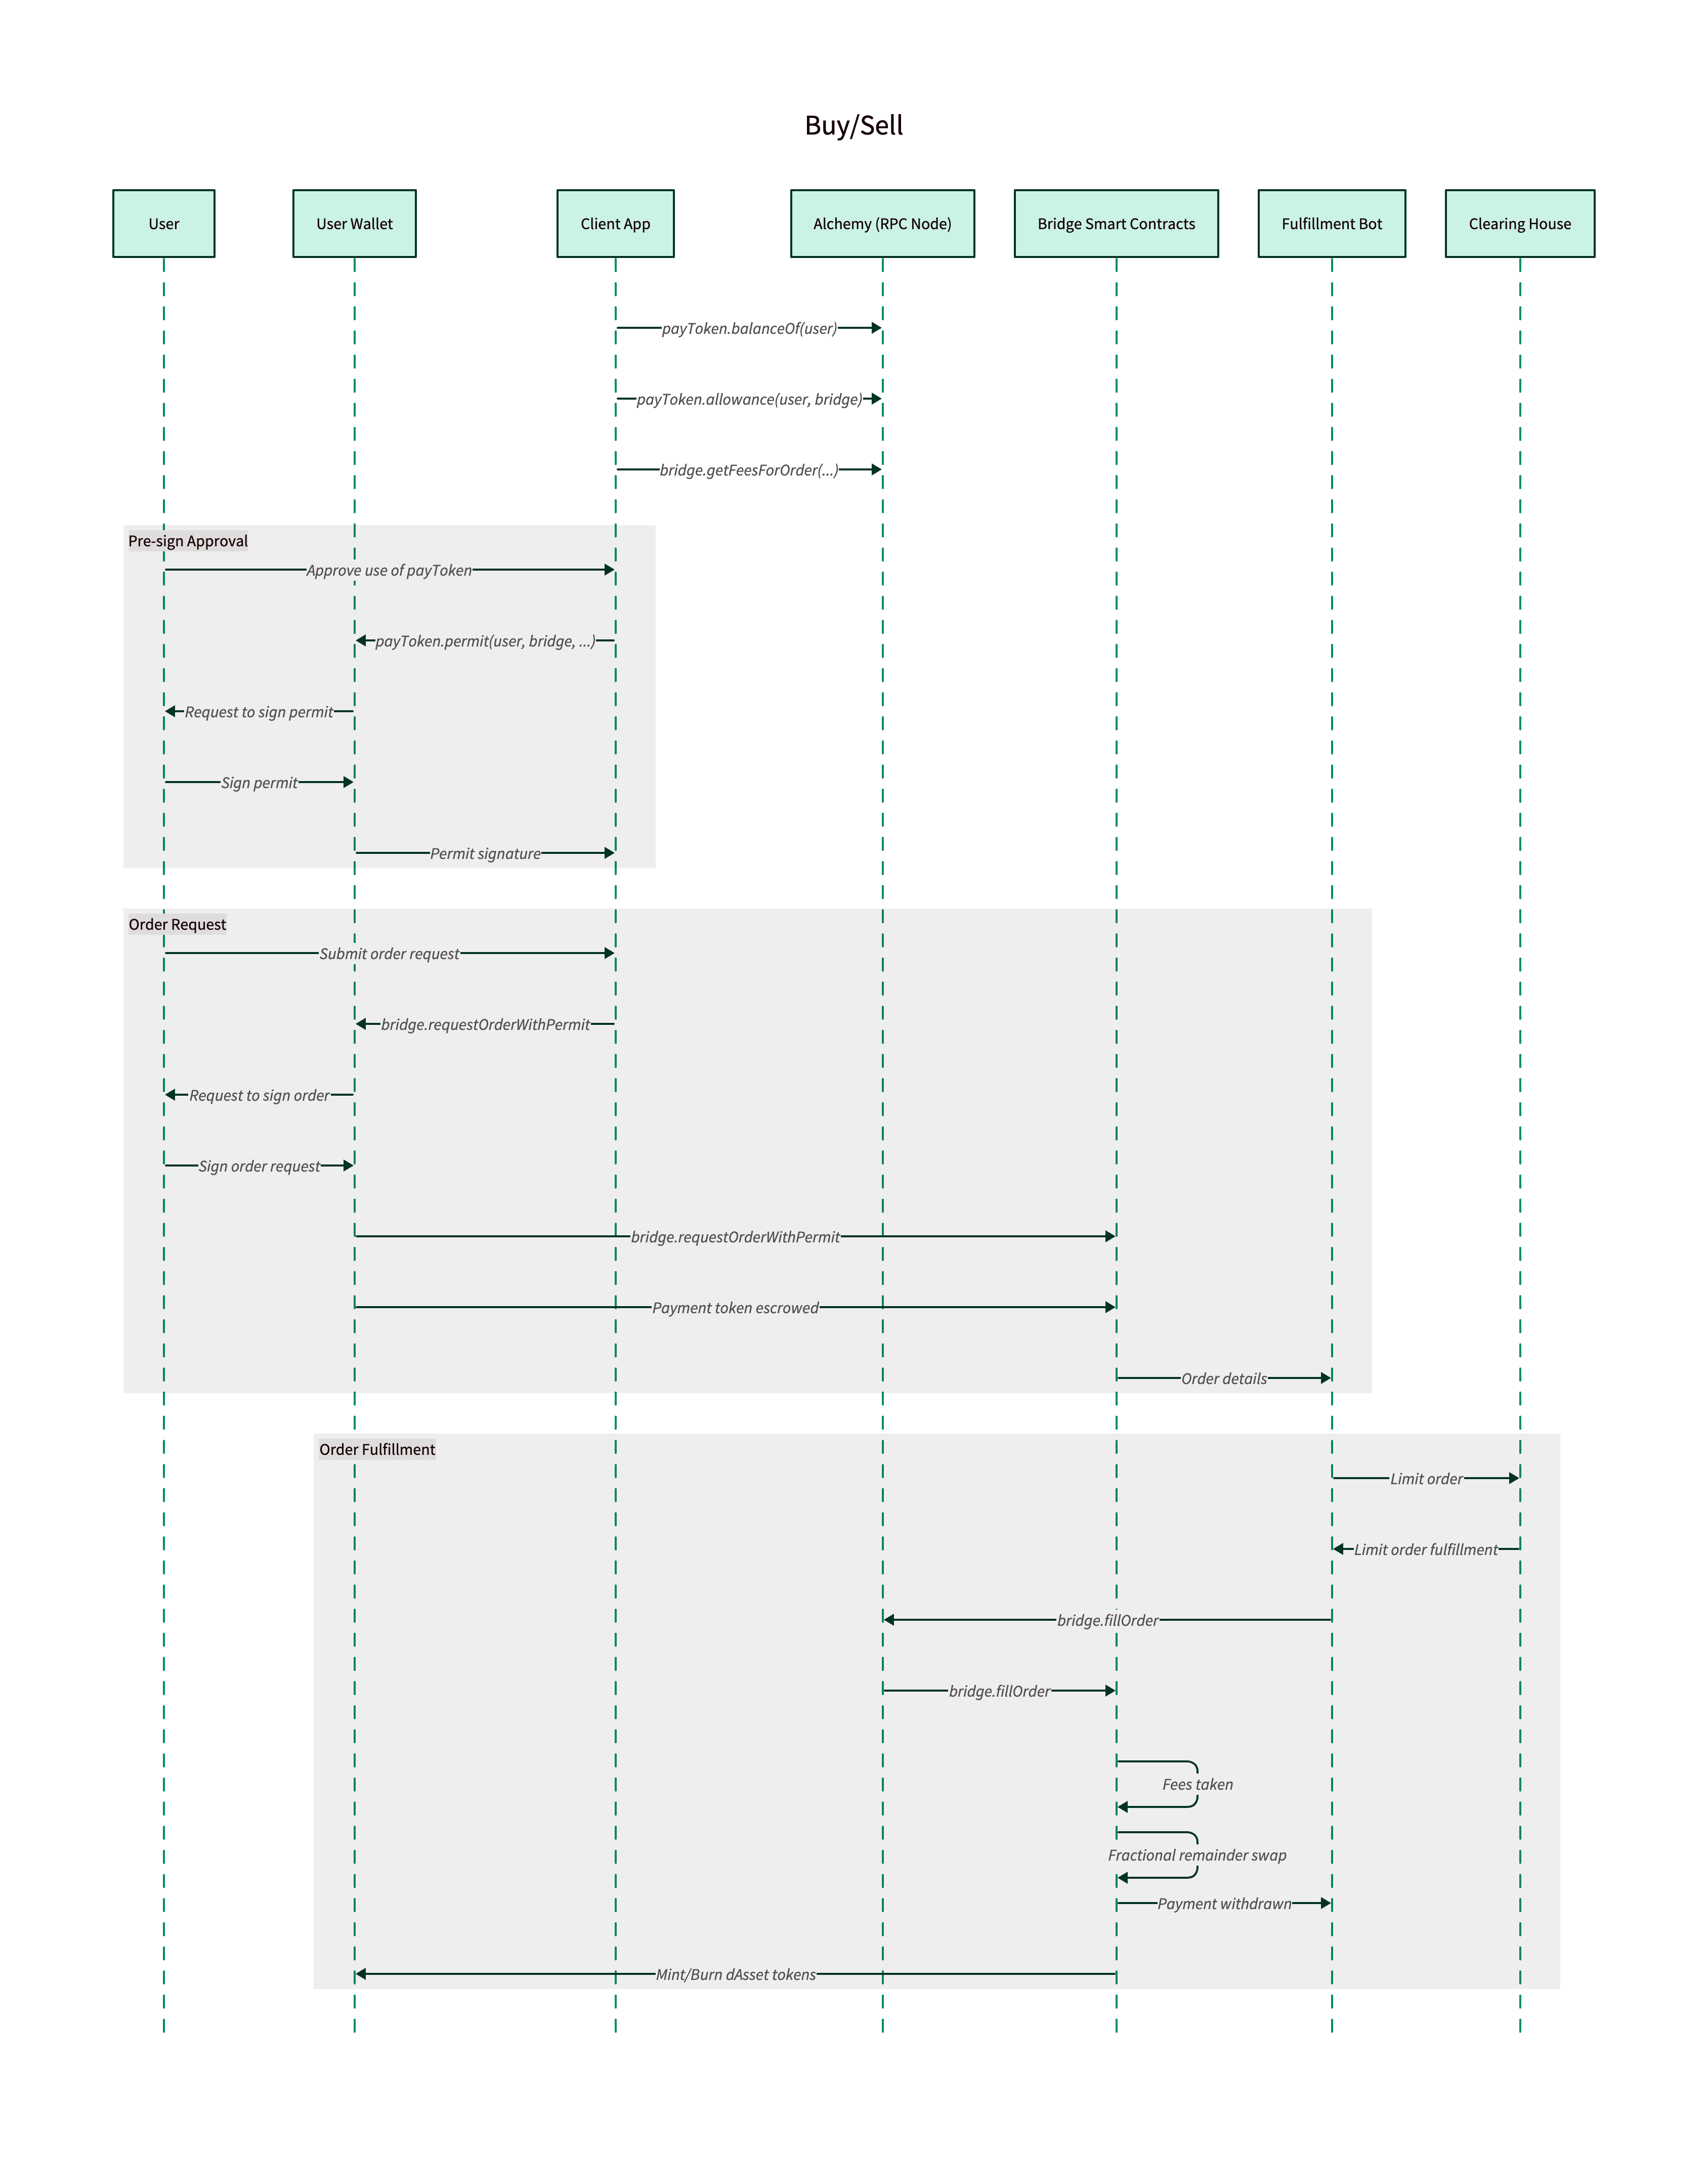
\includegraphics[width = \textwidth]{brokerage-order.d2}
    \caption{Order Processing Sequence Diagram}
  \end{figure}
  \clearpage
  }
  
Orders specify an asset token (the dShare) and a payment token (e.g. USDC). A buy order takes payment token and gives dShares. A sell order takes dShares and gives payment token. 

\subsection{Fees}

Order processor fees include a flat per-order fee and a percentage fee rate on the order amount. These fees are taken from the payment token, from the payment amount for buy orders, or from the raw proceeds of the sale for sell orders.

\section{Summary}
In summary, \dshares is a non-custodial, non-upgradeable, and permissionless AMM protocol. It builds upon the concentrated liquidity model introduced in \textsc{Dinari v3} with customizable pools through hooks. Complementary to hooks are other architectural changes like the singleton contract which holds all pool state in one contract, and flash accounting which enforces pool solvency across each pool efficiently. Some other improvements are native ETH support, ERC-1155 balance accounting, new fee mechanisms, and the ability to donate to in-range liquidity providers.

\bibliographystyle{ACM-Reference-Format}
\bibliography{whitepaper}

\section*{Disclaimer}

This paper is for general information purposes only. It does not constitute investment advice or a recommendation or solicitation to buy or sell any investment and should not be used in the evaluation of the merits of making any investment decision. It should not be relied upon for accounting, legal or tax advice or investment recommendations.  This paper reflects current opinions of the authors. The opinions reflected herein are subject to change without being updated. 

\end{document}
\endinput